\documentclass[slidestop,compress]{beamer}
\usepackage[orientation=portrait,size=custom, width=25, height=24.5, debug]{beamerposter}
\usetheme{simple}

\usepackage{lmodern}
\usepackage[scale=2]{ccicons}

% TODO: 
%   position adjustement
%   change colours
%       

% Watermark background (simple theme)

\begin{document}

\begin{frame}[plain]
\begin{block}{\centering $\pmb \mu$-gravity Controls Testing}
\hspace{1 mm}
\begin{itemize}
\item Bode analysis of cube dynamics in ``space-like" free-fall environment
\item {\it Portland State University's} Dryden Drop Tower facility can access a 1x$10^{-5}$ to $10^{-6}$-g environment for 2.1 s
\item Cube damps roll following a random (25\% duty cycle PWM) perturbing impulse\\
\end{itemize}
\begin{figure}[!ht]
\centering
{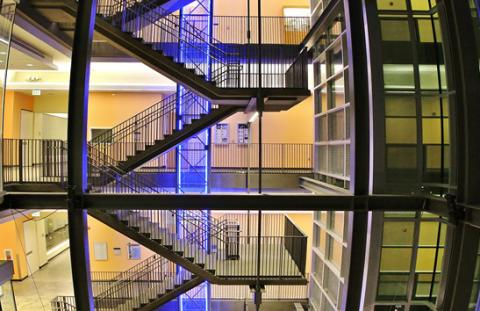
\includegraphics[width=0.9\linewidth]{MCHS-NASA-2016_03.jpg}
\caption{{\it Portland State University's} Dryden Drop Tower (Credit: Andrew Wollman)}
} 
\end{figure}

\end{block}    
\end{frame}

\end{document}

